\documentclass[11pt,letterpaper,boxed]{../hmcpset}
%\let\ifpdf\relax
\usepackage[margin=1in]{geometry}
\usepackage{graphicx}
\usepackage{enumerate}
\usepackage{amsthm}
\usepackage{amsmath}

\newcommand{\ds}{\displaystyle}
\newcommand{\half}{\frac{1}{2}}
\newcommand*\Eval[3]{\left.#1\right\rvert_{#2}^{#3}}
\newcommand{\eval}{\biggr\rvert}
%\renewcommand{\vec}[1]{\mathbf{#1}}
\def\EE{{\cal E}}

\setlength{\parindent}{0cm}

\name{}
\class{Physics 111 Section 1}
\assignment{Problem Set 01}
\duedate{September 5, 2016}

\begin{document}

\problemlist{Calculus of Variations (Reading: Chapter 6)}
\textbf{Help:}

\begin{problem}[i]
By either geometric or mathematical (i.e., represent $\vec r$ in a particular coordinate system and then take a time derivative) arguments, demonstrate that the velocity of a particle in spherical coordinates is given by: $$\vec v = \dot{\vec r} = \dot r \hat r + r \dot \theta \hat \theta + r \sin \theta \dot \phi \hat \phi $$
We could continue to turn the crank on this and get the acceleration in spherical coordinates but I think you get the point: Finding a system's governing equations for an $\vec F = m\vec a$ analysis is, for all but the most straightforward geometries, pretty challenging and coordinate-system dependent.
\end{problem}


\vfill
\begin{solution}




\end{solution}

\newpage

\begin{problem}[6.1 \& 6.16]
Show that a great circle gives the geodesic - shortest path - between two points on the surface of a sphere.\\
From the book:\\

[6.1] The shortest path between two points on a \textit{curved surface}, such as the surface of a sphere is called a \textbf{geodesic}. To find a geodesic, one has first to set up an integral that gives the length of a path on the surface in question. This will always be similar to the integral (6.2) but may be more complicated (depending on the nature of the surface) and may involve different coordinates than $x$ and $y$. To illustrate this, use spherical polar coordinates $(r, \theta, \phi)$ to show that the length of a path joining two points on a sphere of radius $R$ is
$$ L = R\int_{\theta_1}^{\theta_2} \sqrt{1 + \sin^2 \theta \phi' (\theta)^2} \ d \theta $$
if $(\theta_1,\phi_1)$ and $(\theta_2, \phi_2)$ specify the two points and we assume that the path is expressed as $\phi = \phi(\theta)$.\\

[6.16] Use the result (6.41) of Problem 6.1 to prove that the geodesic (shortest path) between two given points on a sphere is a great circle. [\textit{Hint}: The integrand $f(\phi, \phi',\theta)$ in (6.41) is independent of $\phi$, so the Euler-Lagrange equation reduces to $\partial f/\partial \phi' = c$, a constant. This gives you $\phi'$ as a function of $\theta$. You can avoid doing the final integral by the following trick: There is no loss of generality in choosing your $z$ axis to pass through the point 1. Show that with this choice the constant $c$ is necessarily zero, and describe the corresponding geodesics.]


\end{problem}
\begin{solution}


\vfill
\end{solution}

\newpage

\begin{problem}[6.14 \& 6.25]
Show that the parametric brachistochrone equations are equivalent to the cycloid. For part (c), you should find that for the first $x_2, y_2$ we have $\theta = \pi$, and for the second, $x_2, y_2$ pair that $\theta = 2\pi$. Then, show that the brachistochrone is isochronous; you may use Mathematica or some similar package to evaluate the integral.\\
From the book:\\

[6.14]
\textbf{(a)} Prove that the brachistochrone curve (6.26) is indeed a cycloid, that is, the curve traced by a point on the circumference of a wheel of radius $a$ rolling along the underside of the $x$ axis. \textbf{(b)} Although the cycloid repeats itself indefinitely in a succession of loops, only one loop is relevant to the brachistochrone problem. Sketch a single loop for three different values of $a$ (all with the same starting point 1) and convince yourself that for any point 2 (with positive coordinates $x_2, y_2$) there is exactly one value of $a$ for which the loop goes through the point 2. \textbf{(c)} To find the value of $a$ for a given point $x_2, y_2$ usually requires solution of a transcendental equation. Here are two cases where you can do it more simply: For $x_2 = \pi b, y_2 = 2b$ and again for $x_2 = 2\pi b, y_2 = 0$ find the value for $a$ for which the cycloid goes through the point 2 and find the corresponding minimum times.\\

$$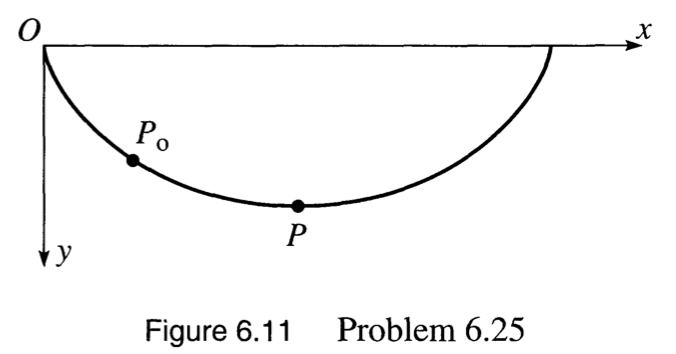
\includegraphics[scale=0.5]{fig611}$$
[6.25] Consider a single loop of the cycloid (6.26) with a fixed value of $a$, as shown in Figure 6.11. A car is released from rest at a point $P_0$ anywhere on the track between $O$ and the lowest point $P$ (that is, $P_0$ has parameter $0< \theta_0 < \pi$). Show that the time for the car to roll from $P_0$ to $P$ is given by the integral
$$ time(P_0 \to P) = \sqrt{\frac{a}{g}} \int_{\theta_0}^\pi \sqrt{\frac{1 - \cos \theta}{\cos \theta_0 - \cos \theta}} \ d\theta$$
and prove that this time is equal to $\pi \sqrt{a/g}$. Since this is independent of the position of $P_0$, the cart takes the same time to roll from $P_0$ to $P$, whether $P_0$ is at $O$, or anywhere between $O$ and $P$, even infinitesimally close to $P$. Explain qualitatively how this surprising result can possibly be true. [\textit{Hint}: To do the mathematics, you have to make some cunning changes of variables. One route is this: Write $\theta = \pi - 2\alpha$ and then use the relevant trig identities to replace the cosines of $\theta$ by sines of $\alpha$. Now substitute $\sin \alpha = u$ and do the remaining integral.]
\end{problem}
\begin{solution}


\vfill
\end{solution}

\newpage

\begin{problem}[6.23]
Minimizing flight time in the presence of wind shear.\\
From the book:\\

[6.23] An aircraft whose airspeed is $v_0$ has to fly from town $O$ (at the origin) to town $P$, which is a distance $D$ due east. There is a steady gentle wind shear, such that $v_{wind} = V y \hat x$, where $x$ and $y$ are measured east and north respectively. Find the path, $y = y(x)$, which the plane should follow to minimize its flight time. as follows: \textbf{(a)} Find the plane's ground speed in terms $v_0, V, \phi$ (the angle by which the plane heads to the north of east), and the plane's position. \textbf{(b)} Write down the time of flight as an integral of the form $\int_0^D f \ dx$. Show that if we assume that $y'$ and $\phi$ both remain small (as is certainly reasonable if the wind speed is not too large), the the integrand $f$ takes the approximate form $f = (1 + \half {y'}^2)/(1 + ky)$ (times an uninteresting constant) where $k = V/v_0$. \textbf{(c)} Write down the Euler-Lagrange equation that determines the best path. To solve it, make the intelligent guess that $y(x) = \lambda x(D-x)$, which clearly passes through the two towns. Show that it satisfies the Euler-Lagrange equation, provided $\lambda = (\sqrt{4 + 2k^2 D^2} -2)/(kD^2)$. How far north does this path take the plane, if $D = 2000$ miles, $v_0 = 500$ mph, and the wind shear is $V = 0.5$ mph/mi? How much time does the plane save by following this path? [You'll probably want to use a computer to do this integral.]

\end{problem}
\begin{solution}


\vfill
\end{solution}

\newpage

\begin{problem}[6.26]
Euler-Lagrange equations for a system with more than one dependent variable.\\
From the book:\\

[6.26] Give in detail the argument that leads from the stationary property of the integral (6.30) to the two Euler-Lagrange equations (6.34).
\end{problem}
\begin{solution}


\vfill
\end{solution}


\end{document}
